\section{VoLTE音视频传输方案}
\label{chap:backinfo:volte}

%VoLTE实现概述

\insertFigure{
	\begin{figure}
		\centering
        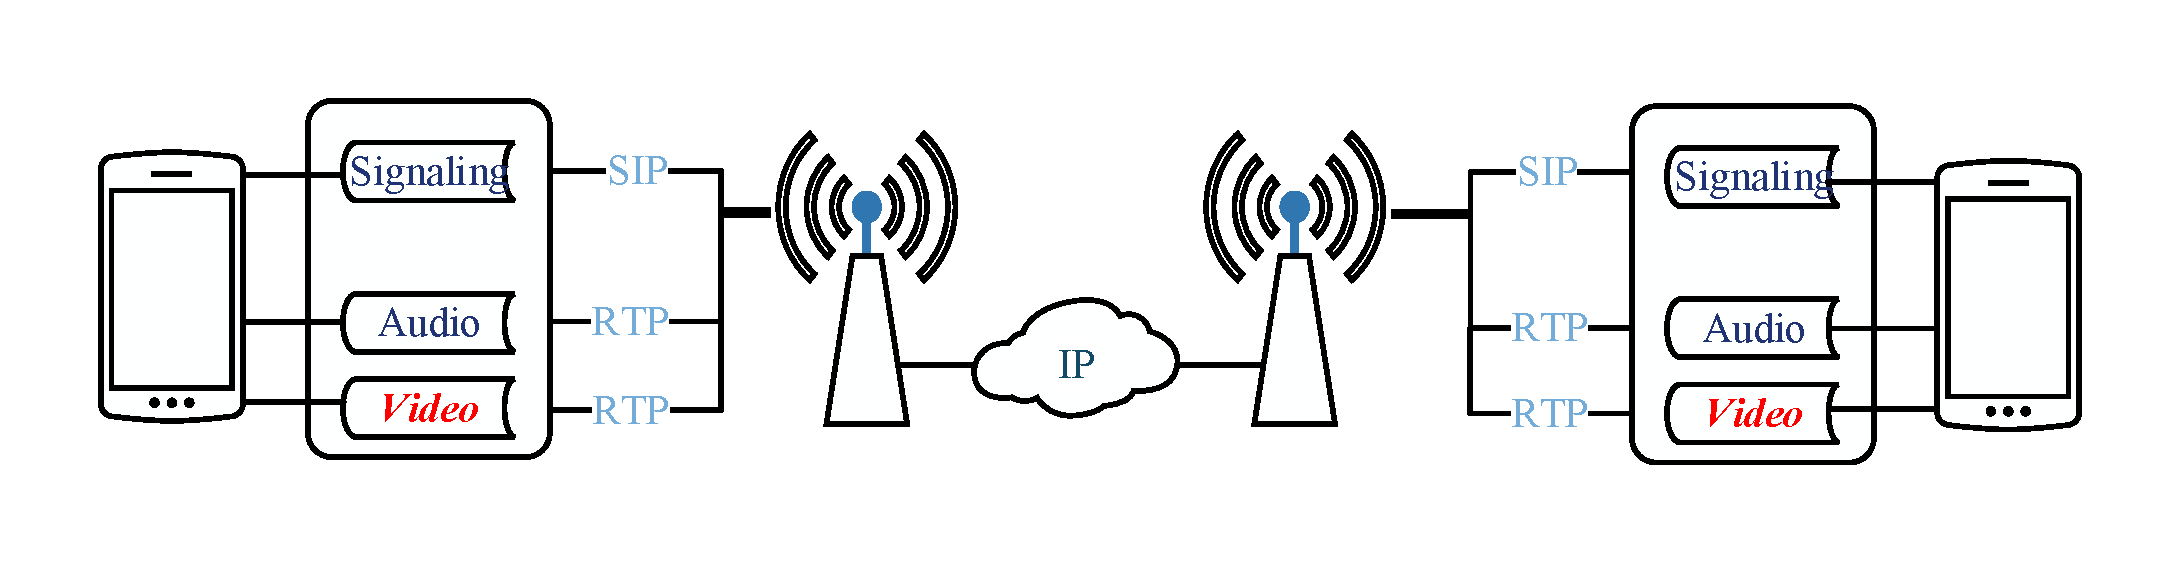
\includegraphics[width=0.95\textwidth]{chapters/chapter2/figures/volte-model.pdf}
        \caption{VoLTE视频通话中的数据流}\label{fig:2:volte-model}
	\end{figure}
}

语音通信功能是移动通信技术的基本需求,随着智能终端的发展,用户的移动数据需求才逐渐占据主流。在移动通信标准中,基于LTE的第四代移动通信技术已经转变为全IP网络,实现了语音主导到数据主导的转换。不同于原有的通信方案,LTE对数据传输进行了优化,同时对音视频通话功能进行了升级。

\subsection{VoLTE数据处理流程}
\label{chap:backinfo:volte:datastream}

在2G及3G时代,基于电路交换音频通话技术,是支撑语音业务的核心解决方案。进入4G时代,核心网络改变为全数据包交换,基于电路交换的音频通话已经无法兼容,需要全新的通话模式。于是,类似于VoIP音视频解决方案,基于LTE的VoLTE成为4G时代的音视频通话方案。在实际应用中,支持VoLTE的终端能够快速建立呼叫,否则将回落到3G或2G网络,从而兼容多种设备及场景。\nupcite{poikselka2012voice}

如图\nref{fig:2:volte-model},VoLTE视频通话过程中,需要三个数据信道,分别为信令信道、语音信道及视频信道,所有的信道均采用数据包进行传输。通过音视频分离方式,VoLTE实现了多场景兼容。通过信令信道,对通话模式及参数进行协商,决定语音信道及视频信道采用的编码方式。相对2G及3G网络,LTE支持的数据上行速率有了显著提升,能够支撑更多的终端进行高清晰度通话。\nupcite{ZHANG201929}

\insertTable{
    \begin{table}
        \centering
        \caption{LTE业务QCI分配表概述}
        \label{tab:2:qci-classification}
        \begin{threeparttable}
            \begin{tabular*}{\textwidth}{@{\extracolsep{\fill}}cccccc}
                \toprule
                QCI分类 & 资源类型 & 优先级 & 可接受延迟 & 可接受丢包率 & 服务类型 \\ 
                \midrule
                1 & 保证QoS & 2 & 100 ms & $10^{-2}$ & VoLTE语音 \\ 
                2 & 保证QoS & 4 & 150 ms & $10^{-3}$ & VoLTE视频 \\
                5 & 不保证QoS & 1 & 100 ms & $10^{-6}$ & VoLTE信令 \\
                7 & 不保证QoS & 7 & 100 ms & $10^{-6}$ & 交互式音视频应用 \\
                \bottomrule
            \end{tabular*}
            \begin{tablenotes}
                \footnotesize
                \item[] QoS指Quality of Service,服务质量
                \item[] QCI指Quality of Service Class Identifiers,QoS分类标签
            \end{tablenotes}
        \end{threeparttable}
    \end{table}
}

相较于固网,移动无线网络受噪声干扰明显,导致用户通话体验变差。如表\nref{tab:2:qci-classification},根据LTE业务分类,VoLTE的信令数据包具有1级最高优先级,可接受时延为{100\ ms},可接受丢包率为$10^{-6}$;VoLTE语音数据包具有2级优先级,可接受时延为{100\ ms},可接受丢包率为$10^{-2}$;VoLTE视频数据包优先级降为4级,可接受时延为{150\ ms},可接受丢包率为$10^{-3}$。另一方面,即使VoIP应用的数据包也是经LTE网络传输,其服务质量也是完全不同的,运营商网络只保证尽力传输。VoIP应用的音视频数据对应的优先级为7,可接受时延为{100\ ms},可接受丢包率为$10^{-6}$。\nupcite{7154042,6996582,Li:2015:IVS:2810103.2813618}

因此,VoLTE相较于其它VoIP应用,受网络调度产生抖动的几率要小。时间隐通道的操作空间较小,对构建方法提出了新的挑战。

\subsection{VoLTE数据包传输特征}
\label{chap:backinfo:volte:packets}
%VoLTE音视频分流处理的模式(分清楚执行组件),结合传输的逻辑设计
通过支持VoLTE的终端设备进行视频通话,参与数据处理的处理器通常由两部分组成。其中一个是AP(Application Processor)也就是应用处理器,另外一个是BP(Baseband Processor)也就是基带处理器。AP参与操作系统中通用数据的处理,BP负责的是无线通信数据的处理,二者相互补充,共同完成智能终端设备的数据处理任务。

\insertFigure{
	\begin{figure}
		\centering
        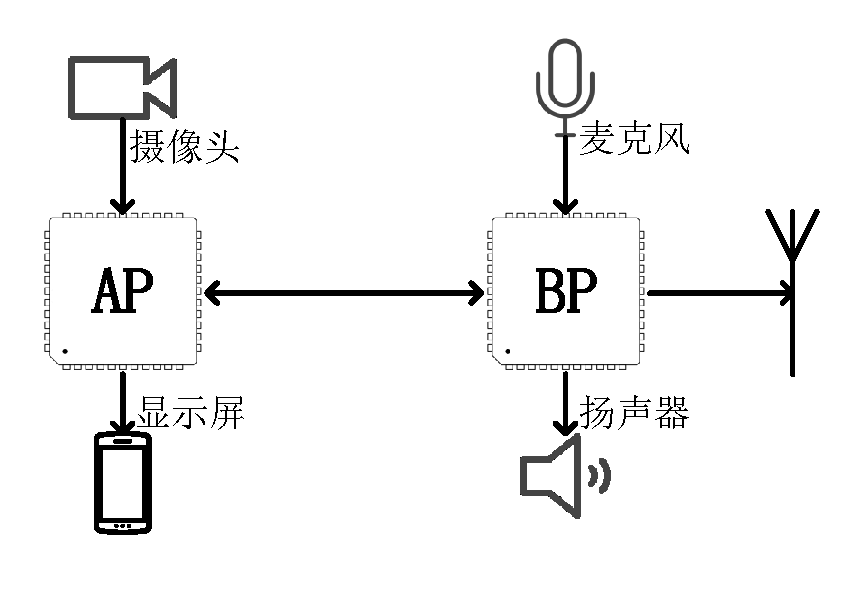
\includegraphics[width=0.55\textwidth]{chapters/chapter2/figures/ap-bp.pdf}
        \caption{VoLTE视频通话时AP与BP功能划分}\label{fig:2:ap-bp}
	\end{figure}
}

如图\nref{fig:2:ap-bp},AP与BP对应不同的媒体类型。对于VoLTE语音数据,由基带处理器按照设定的时间间隔,完成模拟信号的采样、编码,并将打包好的语音数据包通过射频系统传输。对于VoLTE视频数据,由于图像处理模块集成在应用处理器中,视频数据包需要应用处理器参与。应用处理器调用摄像系统驱动,获取编码后的视频数据流,按照视频帧分别进行切片打包,得到RTP视频数据包。视频数据包由系统内核中的协议栈发送,最终由BP通过射频系统传输。类似的,在接收阶段,VoLTE语音数据由基带处理器完成接收、解包、解码,并交由扬声器进行播放。VoLTE视频数据包则交付系统中的网络组件,完成解包、解码后,由通话软件显示在屏幕上。\nupcite{ZHANG201929,guo2019volte}

%抓包结果,分析传输特征,时间间隔、发送密度
\subsubsection{音视频数据包发送特征}
\label{chap:backinfo:volte:packets:send}

\insertFigure{
    \begin{figure}
        \centering
        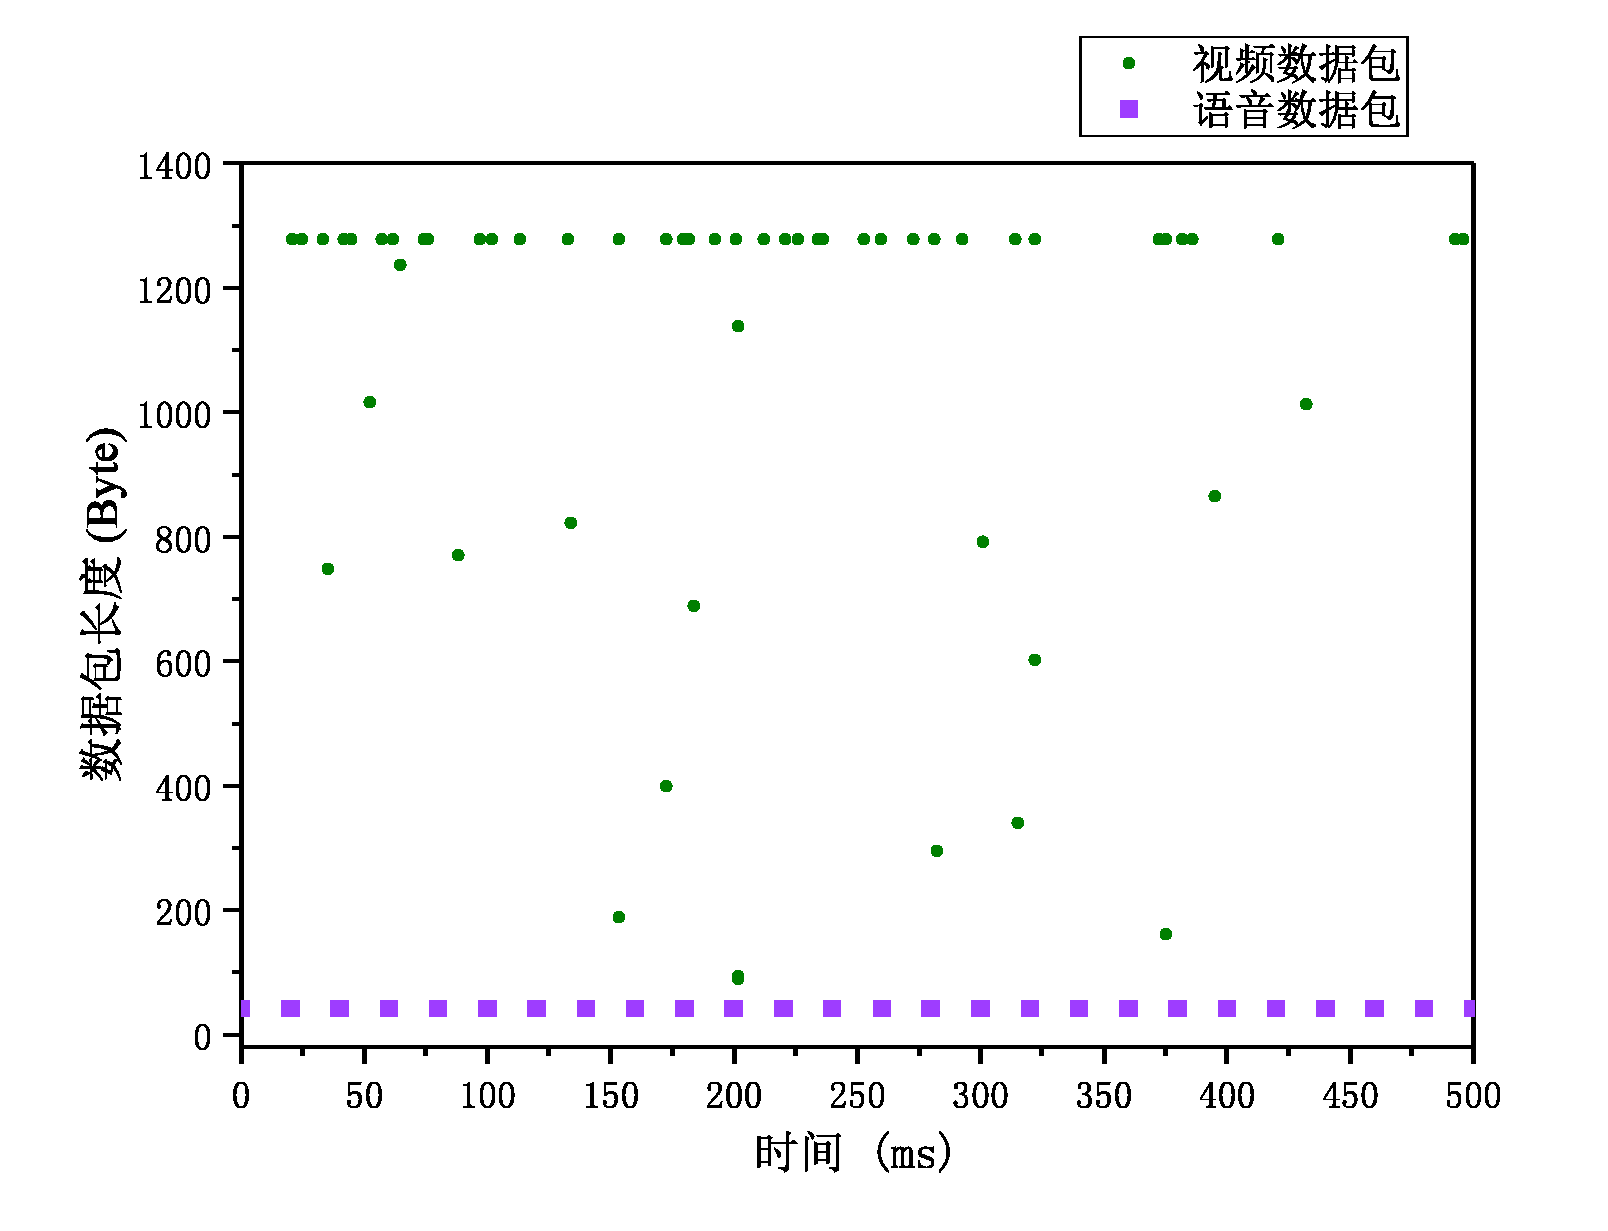
\includegraphics[width=0.8\textwidth]{chapters/chapter2/figures/length-audio-video.pdf}
        \caption{VoLTE音视频数据包发送间隔示意}\label{fig:2:audio-video}
    \end{figure}
    \begin{figure}
        \centering
        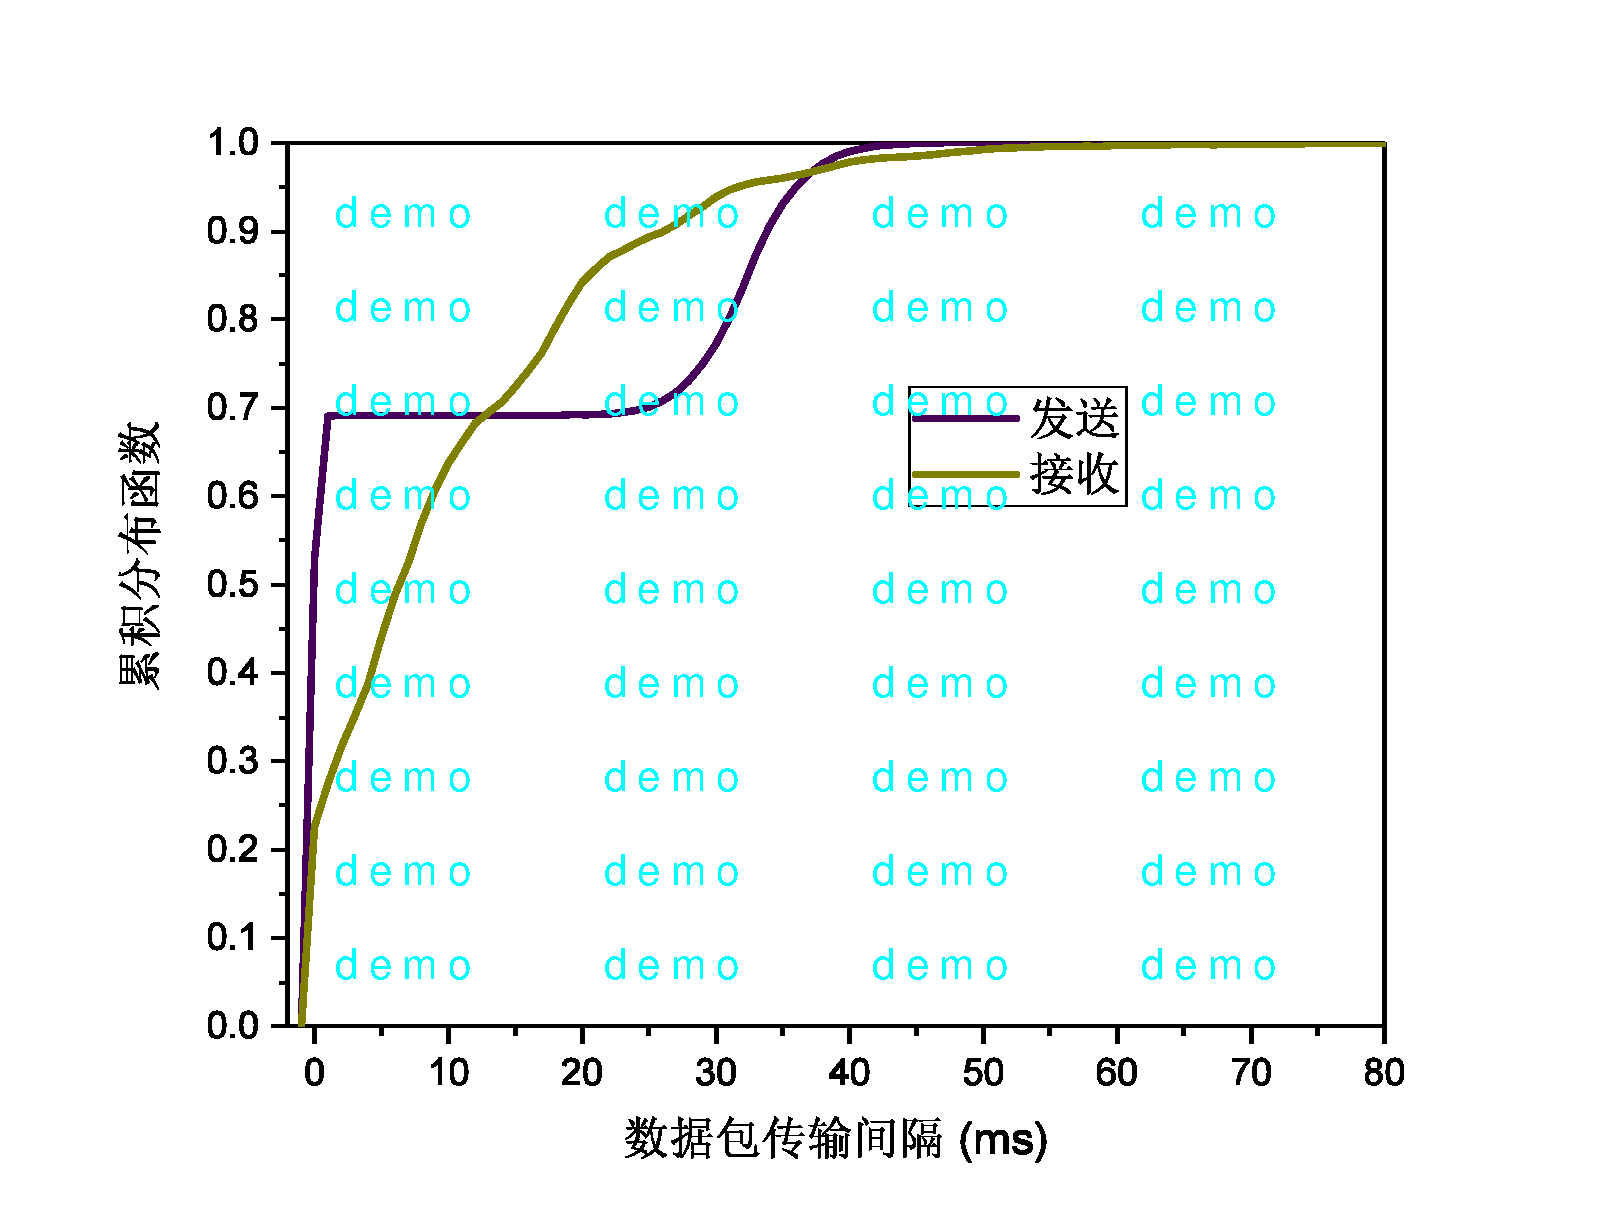
\includegraphics[width=0.8\textwidth]{chapters/chapter2/figures/cdf-send-receive.pdf}
        \caption{VoLTE视频数据包IPD的累积分布函数}\label{fig:2:cdf-ipd}
    \end{figure}
    \begin{figure}
        \centering
        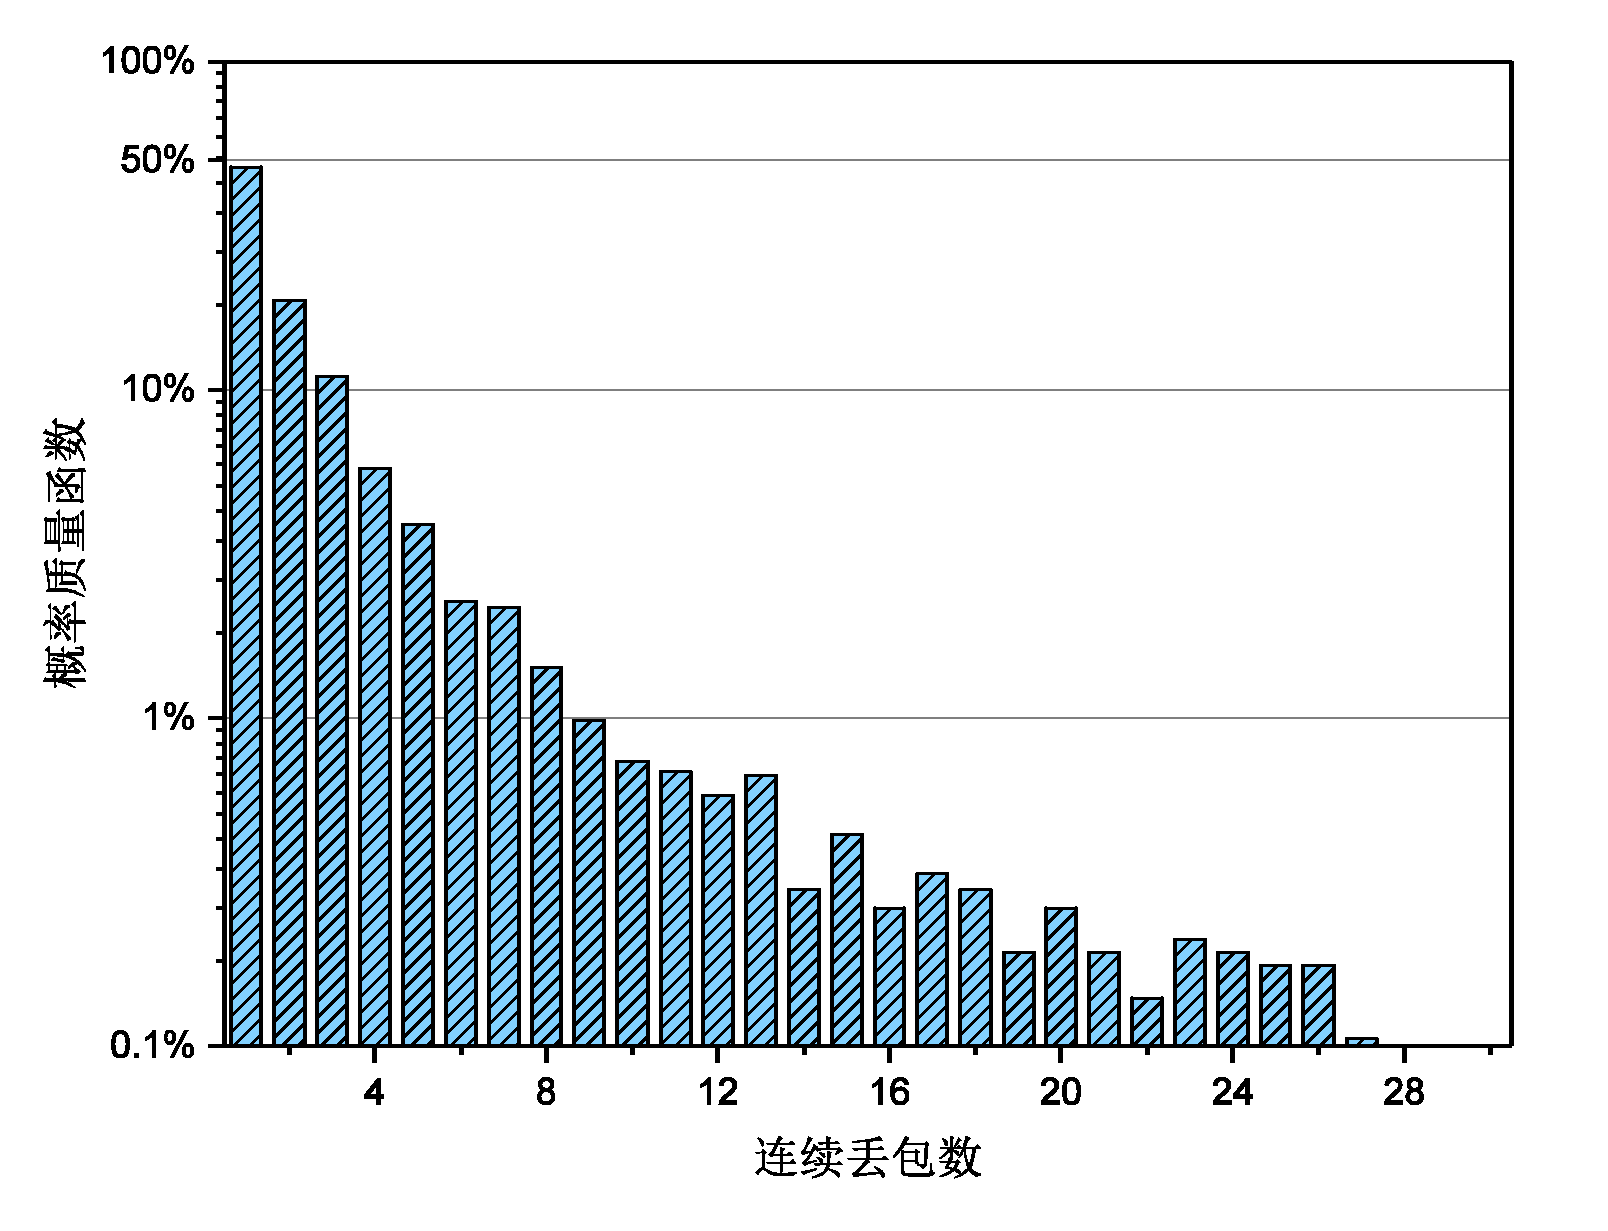
\includegraphics[width=0.8\textwidth]{chapters/chapter2/figures/pmf-dropout.pdf}
        \caption{连续丢包数量的概率质量函数}\label{fig:2:pmf-dropout}
    \end{figure}
}

对于音频数据包,采用AMR-WB(Adaptive Multi-Rate Wideband)格式编码时,数据包在非静音期每{20\ ms}发送一次,在静音期不发送数据包。\nupcite{8288828}对于视频数据包,数据包发送间隔取决于视频刷新率及编码结果,具有很大的不确定性。\nupcite{zhang2019timestamp}如图\nref{fig:2:audio-video},VoLTE视频数据包的长度虽然在{1300\ 字节}左右有集中分布,但仍有部分数据包长度随机变化;另一方面,VoLTE语音数据包的发送间隔具有规律性,相比较视频数据包的聚集现象更普遍。

\subsubsection{视频数据包发送与接收IPD分布特征}
\label{chap:backinfo:volte:packets:ipd}
如\nref{chap:backinfo:volte:packets:send}所述,VoLTE语音数据包的IPD规律性明显,对构建时间隐通道不利。研究VoLTE视频数据包的传输特征,对VoLTE下时间隐通道构造方法的研究具有重要意义,VoLTE视频数据流对噪声敏感度低,便于时间隐通道隐匿在网络噪声中。

如图\nref{fig:2:cdf-ipd},在发送阶段,IPD主要集中在{30\ ms}及{0\ ms}两部分,由于视频刷新率为{30\ fps},每隔{33\ ms}产生一个新的视频帧,而视频帧又有多个数据包组成,造成发送阶段CDF曲线不平滑。在接收阶段,受网络噪声及传输延迟的影响,IPD在$[0,\ 30]$区间内集中分布,CDF曲线趋于平滑。因此,视频数据包在IPD方面,对时间隐通道的容忍性要优于语音数据包。

\subsubsection{VoLTE视频数据包丢包特征}
\label{chap:backinfo:volte:packets:dropout}
对于VoLTE视频数据包,连续丢包数量的概率质量函数如图\nref{fig:2:pmf-dropout}。该统计结果,来自抓包得到的58万条VoLTE视频数据包,包含低噪声及高噪声在内的多种测试场景。PMF(Probability Mass Function)统计结果显示,VoLTE视频数据信道中的丢包事件,主要由单个离散丢包事件组成,连续大量的丢包事件占据的比例非常小。

\subsection{基于主动丢包的时间隐通道构建基础}
\label{chap:backinfo:volte:scheme}
VoLTE出现丢包的原因,主要由于通信终端与基站的空口传输过程。在复杂的无线环境中,发送端与接收端均会出现丢包可能。对于监听者,只有监听了隐通道发送方的终端设备,才有一定几率发现机遇主动丢包的时间隐通道。然而,在隐通道的威胁模型及实际应用中,监听者主要监听的是中间介质,基于主动丢包的时间隐通道,符合VoLTE的传输特征。

通过对VoLTE通话的理论及实际分析测试,在VoLTE场景中构建时间隐通道,尤其是通过主动丢包的方式构建时间隐通道,应当首先选择VoLTE视频信道作为宿主信道。与此同时,主动丢包的构建方式应当模拟离散丢包模式,并且在统计特征方面拟合已知统计结果。另一方面,VoLTE视频信道自身的丢包率,已经超过了QCI的预期丢包率,证明当前VoLTE仍然不能完全保证服务质量,通过主动丢包构建时间隐通道可行。所以,本文选择VoLTE视频信道,作为时间隐通道的宿主信道。